\chapter{Application platform choices: \texttt{Django} and \texttt{PostgreSQL}}\label{chap:django}

\section{Why a web application for lab workflows (upload + annotation together)}
Electron microscopy data are most useful when the raw signals (e.g.\ \texttt{TIFF} images, spectra) and their context (who acquired them, with which settings, on which sample, and for what purpose) are captured together. In practice, however, these two streams often diverge: files accumulate on shared drives while contextual notes sit in lab books or spreadsheets. A web application brings them back into the same place and time. By presenting a form-driven interface in the browser, it allows users to \emph{deposit} raw data and \emph{annotate} it in a single, guided interaction. The form can validate required fields, enforce controlled vocabularies, and provide immediate feedback about missing or inconsistent entries, reducing the need for follow-up and helping the lab converge on shared conventions.

\medskip
\noindent A web application also makes it straightforward to separate human–computer interaction from heavier processing. Once a deposit has been accepted, the server can take over the structured steps needed for durable storage, without holding the user’s browser open. Centralizing uploads likewise enables uniform access control, consistent record-keeping, and the provision of an \emph{application programming interface (API)}\footnote{API: an interface that exposes application capabilities to software clients, allowing automation and integration.} for scripted ingest from acquisition workstations. Finally, a web application can mirror the laboratory’s working practices in its interface and underlying database, so that daily activities map naturally onto durable storage structures. The concrete hierarchy used in this project is described later in Chapter~\ref{chap:deep-dive-app}.

\section{\texttt{Django}: Model–View–Template and project layout}

\texttt{Django} is a Python web framework designed to encourage clear separation of concerns and fast iteration \parencite{DjangoAtAGlance}. Its architectural pattern is called \emph{Model–View–Template (MVT)} \parencite{DjangoFAQMVC}. This separates the application into three main components:

\begin{itemize}
	\item \textbf{Model:} Represents the data layer of the application. Models define the database structure and handle all data-related logic.
	\begin{itemize}
		\item Implemented in Django as Python classes (subclassing \texttt{models.Model}), each mapping to a database table. 
		\item Responsible for creating, reading, updating, and deleting records. 
		\item Typically backed by relational databases such as MySQL, PostgreSQL, or SQLite \parencite{DjangoDatabases}. 
		\item In our project, \texttt{experiment\_manager/models.py} defines models such as \texttt{Project}, \texttt{Proposal}, and \texttt{Sample}. 
		\item Relationships are expressed through foreign keys (e.g. a \texttt{Proposal} belongs to a \texttt{Project}; a \texttt{Sample} belongs to a \texttt{Proposal}), and Django’s ORM enforces these links in the database. 
	\end{itemize}
	
	\item \textbf{View:} Contains the business logic and request handling. A view receives an HTTP request, processes it, and returns an HTTP response.
	\begin{itemize}
		\item Implemented in Django as Python functions or classes (often defined in \texttt{views.py}). 
		\item Interacts with models to retrieve or update data. 
		\item Delegates presentation to a template after preparing the necessary context data \parencite{DjangoViews}. 
		\item In our project, modules such as \texttt{experiment\_manager/views.py}, \texttt{views\_manage.py}, and \texttt{view\_modals.py} handle user actions. 
		\item Examples include displaying dashboards and processing form submissions for new proposals or experiments. 
	\end{itemize}
	
	\item \textbf{Template:} Manages the presentation layer of the application. Templates define how data is displayed to the user.
	\begin{itemize}
		\item Written as HTML files, optionally enriched with the Django Template Language for dynamic content. 
		\item Contain static structure and placeholders/tags where dynamic data is inserted. 
		\item The template engine fills these placeholders using context data from views \parencite{DjangoTemplates}. 
		\item In our project, templates are located in \texttt{experiment\_manager/templates/}, e.g. \texttt{homepage.html} or \texttt{dashboard.html}. 
		\item These templates determine the UI layout and are rendered by views to produce the final HTML pages shown in the browser. 
	\end{itemize}
\end{itemize}

\begin{figure}[h]
	\centering
	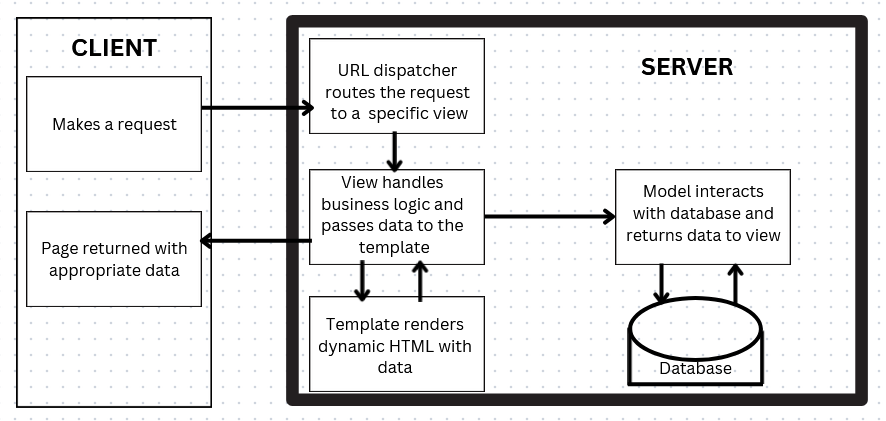
\includegraphics[width=0.7\textwidth]{img/chpt3/django_mvt_diagram.png}
	\caption{Django Model–View–Template (MVT) architecture \parencite{freecodecamp_mvt}.}
\end{figure}

In the MVT workflow, an incoming request is routed by Django’s URL dispatcher (configured in \texttt{urls.py}) to the appropriate view. The \textbf{view} may interact with \textbf{models} to fetch or update data, and then passes that data to a \textbf{template} for rendering into an HTML page. The view finally returns the rendered HTML to the client as an HTTP response \parencite{DjangoRequestResponse,DjangoURLDispatcher}. 

This separation of concerns makes the code more maintainable and reusable: the same model can support multiple views or templates. Django’s design emphasizes the \textbf{Don’t Repeat Yourself (DRY)} principle, keeping logic (views), data access (models), and presentation (templates) decoupled for clarity and reuse \parencite{DjangoPhilosophy}.

\section{Relational databases and the choice of \texttt{PostgreSQL}}

To store and manage the application’s data (such as project info, proposals, 
samples, etc.), we chose a \textbf{relational database} as the backend. 

A \emph{relational database} is a type of database that organizes data into 
tables with rows and columns, and links those tables through defined 
relationships (keys) \parencite{ElmasriNavathe}. In other words, each entity in 
our system (\texttt{Project}, \texttt{Proposal}, \texttt{Sample}, 
\texttt{Experiment}, \texttt{Measurement}) can be represented as a table, and 
relationships (like which samples belong to which proposal) are modeled via 
foreign keys. 

This approach ensures data is stored in a structured way with referential 
integrity – for example, a \texttt{Measurement} record cannot exist without its 
associated \texttt{Experiment}, and an \texttt{Experiment} is linked to a 
\texttt{Sample}, and so on, maintaining a hierarchy. 

\medskip

Relational databases use the SQL language for querying and manipulating data, 
which is a well-established standard for database 
operations \parencite{ElmasriNavathe}. 

We opted for a relational database because our data is highly structured and 
interrelated. The hierarchical nature of projects→proposals→samples→experiments 
lends itself well to the relational model – we can enforce that hierarchy 
through foreign key constraints and ensure consistency (e.g., preventing a user 
from creating an \texttt{Experiment} without specifying its parent 
\texttt{Sample}). 

\medskip

Relational databases also provide \textbf{ACID} properties (Atomicity, 
Consistency, Isolation, Durability), which guarantee reliable transactions and 
consistency of data – an important factor when lab users are uploading and 
annotating critical experiment data \parencite{PostgresAbout}. 

Using a robust DBMS (Database Management System) allows multiple users to 
collaborate and access data concurrently with safety mechanisms for concurrent 
writes and reads. 

\medskip

\noindent
\textbf{Django’s database support:} Django is designed to work with relational 
databases out of the box. It officially supports several popular SQL databases, 
including:
\begin{itemize}
	\item PostgreSQL, 
	\item MySQL (and its fork MariaDB), 
	\item Oracle, 
	\item SQLite \parencite{DjangoDatabases}.
\end{itemize}

By default, a new Django project is often configured with SQLite (a lightweight 
file-based database) for convenience in development. SQLite requires no 
separate server and is great for testing or prototyping, but it is not ideal 
for multi-user production use due to its limitations in concurrency and 
scale \parencite{SQLiteAppropriateUses}. 

For a production environment and for handling potentially large volumes of 
data, a more robust client-server database is preferable. Django makes it 
straightforward to switch the database engine since the model layer is 
abstracted – you simply change the database configuration in 
\texttt{settings.py} and run migrations, without having to rewrite model 
code \parencite{DjangoMigrations}. 

\medskip

In our case, we use SQLite for quick local tests (because it’s simple and 
requires no setup), but for the deployed application we use a dedicated 
relational database server.

\subsection{Choosing PostgreSQL as the database backend} 

After evaluating the options, we decided to use \textbf{PostgreSQL} as the database backend for our application. PostgreSQL (often simply “Postgres”) is a powerful open-source relational database system known for its reliability and rich feature set \parencite{PostgresAbout}. Below are the key reasons for this choice: 

\begin{itemize} 
	\item \textbf{Reliability and integrity:} 
	\begin{itemize}
		\item Proven architecture with a long track record of stability \parencite{PostgresAbout}. 
		\item Fully ACID-compliant for decades, ensuring safe concurrent transactions. 
		\item Reduces the risk of data corruption (e.g. experiment annotations and metadata). 
		\item Can be trusted to faithfully record uploads and form submissions. 
	\end{itemize}
	
	\item \textbf{Advanced feature set:} 
	\begin{itemize}
		\item Supports complex queries and a wide range of data types (including JSON for semi-structured data). 
		\item Built-in full-text search capabilities \parencite{PostgresJSON,PostgresFTS}. 
		\item Highly extensible through user-defined functions and extensions (e.g. PostGIS). 
		\item Strong adherence to SQL standards, making it a future-proof choice \parencite{PostgresAbout}. 
	\end{itemize}
	
	\item \textbf{Scalability and performance:} 
	\begin{itemize}
		\item Efficiently handles large datasets and many concurrent users \parencite{PostgresAbout}. 
		\item Scales well as the number of experiments and users grows. 
		\item Optimizations include indexing, query planning, and replication support. 
		\item Solid performance for both read-heavy and write-heavy workloads, with tools for tuning and optimization. 
	\end{itemize}
	
	\item \textbf{Community support and Django recommendation:} 
	\begin{itemize}
		\item Free and open-source, with decades of active community development. 
		\item Widely recommended within the Django ecosystem for production deployments. 
		\item Django creators highlight PostgreSQL as the most balanced backend in terms of cost, features, speed, and stability \parencite{DjangoDatabases,DjangoPostgresFields}. 
		\item Many Django features (e.g. \texttt{JSONField}, GIS support) work best with PostgreSQL \parencite{DjangoPostgresFields}. 
		\item Rich ecosystem of documentation, examples, and community plugins tailored for Django + PostgreSQL. 
	\end{itemize}
\end{itemize} 

The configuration is straightforward – we installed the \texttt{psycopg2} adapter (which allows Django to talk to Postgres) and updated our \texttt{DATABASES} setting in Django to use the \texttt{django.\allowbreak db.\allowbreak backends.\allowbreak postgresql} engine with the appropriate credentials. Django handles the rest through its object–relational mapping system, so all our data models defined in Python were automatically translated into PostgreSQL tables via migrations. Overall, PostgreSQL provides a solid foundation for storing the application’s critical data, offering both peace of mind (in terms of reliability) and powerful capabilities if we need them down the road.

\subsection{Django’s ORM (Object-Relational Mapper)} 

One of Django’s most powerful features is its 
\textbf{Object-Relational Mapper (ORM)}, which bridges the gap between our 
Python code and the relational database. The Django ORM is an abstraction 
layer that allows developers to interact with the database using Python 
classes and methods instead of writing raw SQL queries \parencite{DjangoORMQueries}. 

In practice, this means we define our data models as Python classes (in 
\texttt{models.py}), and Django will automatically generate the necessary SQL 
to create tables, insert or retrieve records, and so on. For example, a 
simplified version of a model in our app might look like: 

\begin{verbatim}
	class Proposal(models.Model): 
	title = models.CharField(max_length=100) 
	project = models.ForeignKey(Project, on_delete=models.CASCADE) 
	date_created = models.DateTimeField(auto_now_add=True) 
	# ... other fields
\end{verbatim}

When we run Django’s migrations, the ORM translates this model definition into 
a SQL \texttt{CREATE TABLE} statement in PostgreSQL. The table will have 
columns for each field (\texttt{title}, \texttt{project\_id}, 
\texttt{date\_created}, etc.). 

The \texttt{ForeignKey} to \texttt{Project} tells Django (and the database) 
that each \texttt{Proposal} is related to a \texttt{Project}. The ORM enforces 
this relationship at the database level (e.g., by preventing a proposal from 
existing without a valid project reference, thanks to PostgreSQL’s foreign key 
constraints). 

Importantly, we did not have to write any SQL by hand; Django’s migration 
system and ORM handled it for us. This approach improves productivity and 
reduces the likelihood of errors. By eliminating the need to write manual SQL 
queries for most operations, the ORM helps \textbf{reduce errors and speed up 
	development}, allowing us to focus on business logic rather than database 
syntax \parencite{DjangoORMQueries}. 

\medskip

\noindent
\textbf{Typical operations with the ORM:}
\begin{itemize}
	\item Create a new object with \texttt{Proposal.objects.create(...)}.
	\item Query records with methods like \texttt{.filter()} or \texttt{.all()}.
	\item Update by modifying attributes and calling \texttt{.save()}.
	\item Delete with \texttt{.delete()}.
\end{itemize}

Under the hood, Django translates these high-level operations into optimized 
SQL queries. For instance, 
\texttt{Proposal.objects.filter(title\_\_icontains="test")} becomes a 
\texttt{SELECT} query with a \texttt{WHERE} clause in SQL. 

The developers using our codebase don’t need to know SQL dialect differences 
or complex joins; Django ORM takes care of that. It even provides an API for 
traversing relationships. For example: retrieving all \texttt{Experiments} for 
a given \texttt{Project} can be as simple as 
\texttt{project.experiment\_set.all()}. The ORM translates this into the 
appropriate SQL join. 

\medskip

\noindent
\textbf{Benefits of Django’s ORM:}
\begin{enumerate}
	\item \textbf{Database independence} – since our code is not tied to a 
	specific SQL syntax, we can switch the underlying database engine (e.g., 
	SQLite to PostgreSQL) with minimal changes \parencite{DjangoORMQueries}. 
	This is useful in our cycle: tests run on SQLite, deployment uses PostgreSQL.
	
	\item \textbf{Security} – Django automatically escapes parameters to 
	protect against SQL injection \parencite{DjangoSecurity}.
	
	\item \textbf{Integration with Django components} – once a model is 
	defined, Django can auto-generate an admin interface and forms for it, 
	without extra SQL work \parencite{DjangoAdmin}.
	
	\item \textbf{Support for complex lookups and relationships} – we can 
	express advanced queries in a readable way. If needed, we still have the 
	option to write raw SQL or use lower-level cursors, but so far the ORM has 
	been sufficient \parencite{DjangoRawSQL}.
\end{enumerate}
